\section{Numerical illustrations}\label{sec-verify}

This section illustrates large fixed dictionaries with Horseshoe shrinkage in finite samples. It addresses three questions: how Horseshoe shrinkage compares with dense Gaussian shrinkage on the same dictionary (Section~\ref{sec:benchmarks}), whether the empirical error decay reflects the sparsity-driven rates of Section~\ref{sec:method} (Section~\ref{sec:convergence}), and how one fixed rule for the dictionary and the prior performs on real series of very different complexity (Section~\ref{sec:applications}). In every example, once $n$, the growth exponent $b$, and the basis are fixed, the dictionary evaluated at the design points is a fixed design matrix with $n$ rows and one column per dictionary element, and posterior computation is that of a Bayesian linear regression under a Horseshoe prior. All Markov chain Monte Carlo runs use the Gibbs sampler of the \texttt{horseshoe} package in \texttt{R} \citep{HorseshoeR}.

\subsection{Finite-sample comparison across benchmark functions}\label{sec:benchmarks}

We consider three periodic regression functions on $[0,1]$, built from
rectified sines:
\begin{align*}
f_1(x)&=\tfrac12\,|\sin(\pi(x-0.5))|,\\
f_2(x)&=|\sin(\pi(x-0.3))|^3+0.7\,|\sin(\pi(x-0.7))|^3,\\
f_3(x)&=|\sin(\pi(x-0.2))|^5+|\sin(\pi(x-0.5))|^5+0.6\,|\sin(\pi(x-0.9))|^5.
\end{align*}
Each factor $|\sin(\pi(x-x_0))|$ is $1$-periodic and smooth except for a single cusp at $x=x_0$; raising it to an odd power $p$ makes the target $C^{p-1,1}$ at that cusp and $C^\infty$ elsewhere. Under the integer Lipschitz--H\"older convention $C^m=C^{m-1,1}$, the nominal regularities are therefore $m=1,3,5$, with kinks in derivatives of orders $0$, $2$, and $4$, respectively.

For each benchmark, observations are generated on an equally spaced grid from the Gaussian regression model~\eqref{eq:model}, with noise standard deviations $0.15$, $0.07$, and $0.10$ for $f_1,f_2,f_3$, respectively. The comparison uses $n=1000$ and
\begin{align*}
J_n=\lfloor n^{0.7}\rfloor=125,
\end{align*}
the number of columns of the real Fourier dictionary: the constant, sine--cosine pairs, and, when $J_n$ is even, one further cosine. The noise variance is treated as known. The prior is the Horseshoe of \citet{Carvalho2009} with a shared half-Cauchy global scale; the point estimate is the coefficientwise posterior mean, computed from $5{,}000$ draws after $1{,}000$ burn-in iterations.

As a dense benchmark with global $\ell_2$ shrinkage, we fit ridge regression. Ridge regression is the posterior mean under the Gaussian prior $\theta_j\overset{\mathrm{iid}}{\sim}N(0,\sigma^2/\lambda)$, so it is the natural dense counterpart of the Horseshoe: the Gaussian prior applies the same penalty to every coefficient, whereas the Horseshoe shrinks small coefficients strongly and leaves large ones nearly untouched. With $X\in\mathbb{R}^{n\times J_n}$ the design matrix,
\[
\widehat\theta_{\mathrm{ridge}}
=\arg\min_{\theta}\left\{\|Y-X\theta\|_2^2+\lambda\|\theta\|_2^2\right\},
\]
where the penalty includes the constant coefficient and $\lambda$ is selected by 20-fold cross-validation over a grid of $160$ values \citep{Arlot2010,Krstajic2014}. Both methods use the same dictionary, so the comparison isolates the effect of the prior: global--local Horseshoe shrinkage versus dense Gaussian shrinkage.

\begin{figure}[ht]
\centering
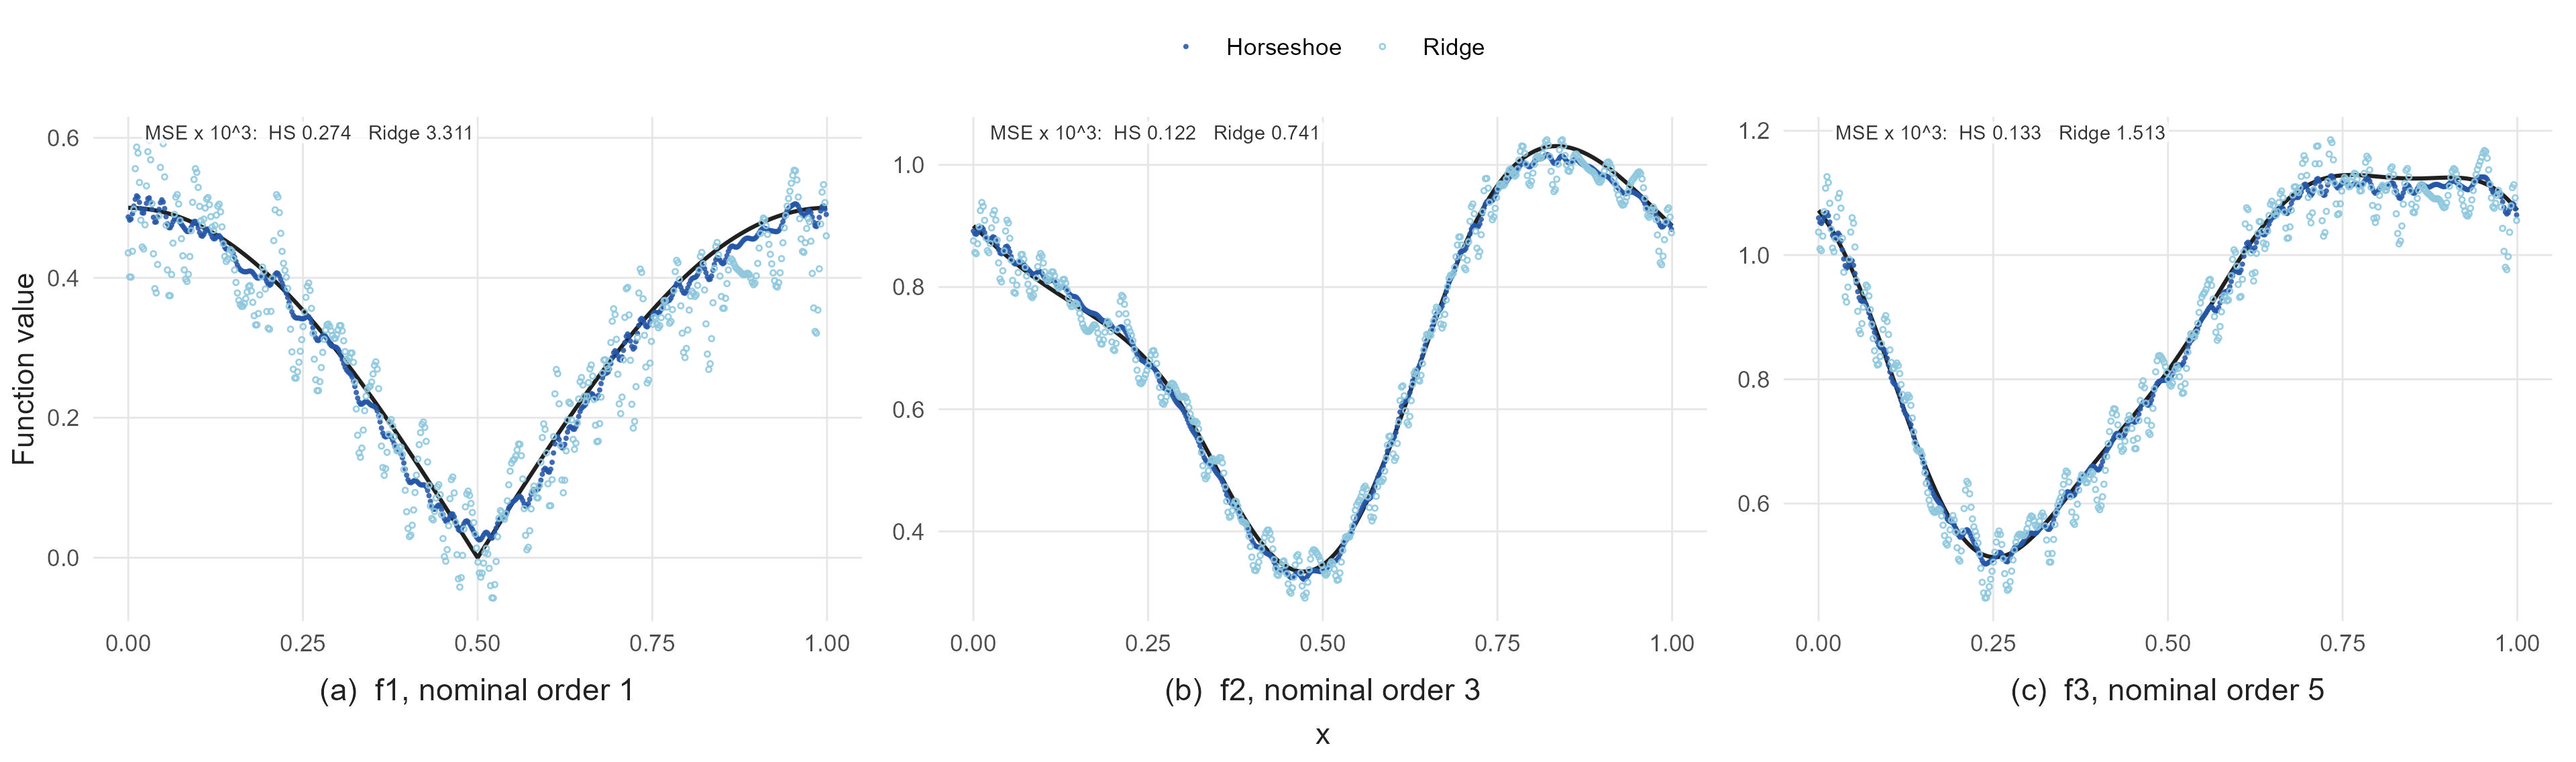
\includegraphics[width=\textwidth]{Ridge_Hs/ridge_hs_trend_comparison.jpg}
\caption{Fourier fits for the three benchmark functions in one simulated data set.  The black curves are the true functions, the dark-blue filled points are the Horseshoe posterior means, and the light-blue open points are the cross-validated ridge estimates.  The in-panel annotations report design-point MSE multiplied by $10^3$.  All panels use $n=1000$ and $J_n=\lfloor n^{0.7}\rfloor=125$.}
\label{fig:fourier-estimates}
\end{figure}

Figure~\ref{fig:fourier-estimates} shows one realization. At $J_n=125$, the Horseshoe and ridge MSE values, multiplied by $10^3$, are $0.274$ and $3.311$ for $f_1$, $0.122$ and $0.741$ for $f_2$, and $0.133$ and $1.513$ for $f_3$, so the Horseshoe error is roughly six to twelve times smaller. The Horseshoe estimates stay closer to the target curves, while the ridge estimates show larger local deviations, especially for $f_1$ and $f_3$.

We next hold $n=1000$ fixed and vary the Fourier dictionary size over
$J_n\in\{140,160,\ldots,300\}$. For a fitted curve $\widehat f$, the design-point error is
\begin{align*}
\operatorname{MSE}(\widehat f)
=\frac1n\sum_{i=1}^n\{\widehat f(x_i)-f_0(x_i)\}^2.
\end{align*}

\begin{table}[ht]
\centering
\small
\setlength{\tabcolsep}{3pt}
\caption{Design-point MSE, multiplied by $10^3$, across Fourier dictionary sizes; one simulated response per target, reused for every $J_n$. Boldface marks the lower value in each pair.}
\label{tab:mse}
\begin{tabular}{llrrrrrrrrr}
\toprule
 & & \multicolumn{9}{c}{Dictionary size $J_n$} \\
\cmidrule(lr){3-11}
$f$ & Method
& 140 & 160 & 180 & 200 & 220 & 240 & 260 & 280 & 300 \\
\midrule
\multirow{2}{*}{$f_1$}
& Horseshoe
& \textbf{0.285} & \textbf{0.315} & \textbf{0.294} & \textbf{0.302} & \textbf{0.294} & \textbf{0.299} & \textbf{0.276} & \textbf{0.271} & \textbf{0.279} \\
& Ridge
& 3.746 & 4.245 & 4.714 & 5.150 & 5.579 & 5.982 & 6.440 & 6.819 & 7.383 \\
\midrule
\multirow{2}{*}{$f_2$}
& Horseshoe
& \textbf{0.126} & \textbf{0.131} & \textbf{0.130} & \textbf{0.133} & \textbf{0.128} & \textbf{0.133} & \textbf{0.130} & \textbf{0.129} & \textbf{0.131} \\
& Ridge
& 0.844 & 0.968 & 1.083 & 1.194 & 1.304 & 1.404 & 1.525 & 1.625 & 1.782 \\
\midrule
\multirow{2}{*}{$f_3$}
& Horseshoe
& \textbf{0.140} & \textbf{0.153} & \textbf{0.145} & \textbf{0.151} & \textbf{0.142} & \textbf{0.146} & \textbf{0.138} & \textbf{0.127} & \textbf{0.136} \\
& Ridge
& 1.723 & 1.983 & 2.209 & 2.443 & 2.659 & 2.871 & 3.115 & 3.320 & 3.640 \\
\bottomrule
\end{tabular}
\end{table}

On the $10^3\times\operatorname{MSE}$ scale of Table~\ref{tab:mse}, the Horseshoe values range from $0.271$ to $0.315$, from $0.126$ to $0.133$, and from $0.127$ to $0.153$ for $f_1,f_2,f_3$, respectively, while the ridge values range from $3.746$ to $7.383$, from $0.844$ to $1.782$, and from $1.723$ to $3.640$. The ridge error grows steadily with $J_n$, roughly doubling between $J_n=140$ and $J_n=300$, whereas the Horseshoe error stays essentially flat: over this range, enlarging the dictionary does not hurt the Horseshoe, which is exactly the behavior the large series prior relies on. The Horseshoe has the lower error in all $27$ comparisons.

\subsection{Empirical scaling of point estimators}\label{sec:convergence}

The scaling experiment uses three periodic targets of nominal regularity $m=1,3,5$, labelled $f_1,f_2,f_3$ in Table~\ref{tab:convergence}, with $J_n=\lfloor n^{0.7}\rfloor$ and the sample sizes $n=1000,1500,\ldots,20000$. Two numerical bases are used: the cosine basis $1,\cos(\pi x),\ldots,\cos(\pi J_nx)$, with $J_n+1$ columns, and a single-resolution cubic B-spline basis with $J_n$ columns and equally spaced knots. Posterior inference uses the Horseshoe with a practical global scale rather than the $\tau_n$ of Section~\ref{sec:contraction} (Remark~\ref{rem:practical}), and treats $\sigma^2$ as known. For each $n$, independent data sets are generated; in each, the coefficientwise posterior mean is reconstructed as a function and its error is measured by
\begin{align*}
\operatorname{RMSE}(\widehat f)=\|\widehat f-f_0\|_{2,n},
\end{align*}
the square root of the design-point MSE of Section~\ref{sec:benchmarks}, so that slopes are on the scale of $\epsilon_n$. At each $n$, the RMSE values are summarized by their median across data sets.

\subsubsection{Rate-scale comparison}

For each function and basis, we regress the logarithm of the median RMSE on $\log n$. Under the hypotheses of Remark~\ref{rem:polynomial}, $\epsilon_n\asymp\sqrt{\log n}\,n^{(\gamma-1)/2}$; we therefore also report the slope for the response $\log(\operatorname{RMSE})-\tfrac12\log\log n$. 

\subsubsection{Thresholded coefficient counts}

For data set $\ell$, define the coefficient count
\begin{align*}
\widehat q_{n,\ell}
=\sum_{j}
\mathbf 1\!\left\{|\widehat\theta^{\,\mathrm{mean}}_{j,n,\ell}|>\frac1{J_n}\right\},
\end{align*}
where the sum runs over all columns of the basis. We take its median across data sets and denote by $\widehat\gamma_q$ the slope from regressing $\log\widehat q_n$ on $\log n$. The count $\widehat q_n$ is our estimate of the sparsity level. In the theory, a coefficient is non-negligible when it exceeds $\delta_n=c_\delta\en/J_n=o(1/J_n)$, a threshold calibrated to the strong shrinkage of the theoretical global scale $\tau_n$. Scales that small make the Gibbs sampler numerically unstable for large $n$; in our runs, instability appears once $\tau$ falls much below $1/J_n^{2}$. The practical scale therefore shrinks less, and we use the correspondingly larger threshold $1/J_n$. For the same reason, $\widehat\gamma_q$ is an empirical proxy for the sparsity exponent $\gamma$ of Remark~\ref{rem:polynomial} rather than an estimate of the $a_n$ of Assumption~\ref{ass:sparse}.

\begin{table}[ht]
\centering
\caption{Empirical log--log slopes for the coefficient-wise posterior mean on the grid $n=1000,1500,\ldots,20000$. Raw: response $\log(\mathrm{RMSE})$. Adjusted: response $\log(\mathrm{RMSE})-\tfrac12\log\log n$. $\widehat\gamma_q$: slope of the $1/J_n$ coefficient count. Implied: the exponent $(\widehat\gamma_q-1)/2$ of Remark~\ref{rem:polynomial} evaluated at $\gamma=\widehat\gamma_q$.}
\label{tab:convergence}
\begin{tabular}{llcccc}
\toprule
$f$ & Basis & Raw & Adjusted & $\widehat\gamma_q$ & Implied \\
\midrule
\multirow{2}{*}{$f_1$ ($m=1$)}
& B-spline & $-0.151$ & $-0.210$ & $0.707$ & $-0.147$ \\
& Cosine   & $-0.332$ & $-0.390$ & $0.241$ & $-0.380$ \\
\midrule
\multirow{2}{*}{$f_2$ ($m=3$)}
& B-spline & $-0.145$ & $-0.203$ & $0.718$ & $-0.141$ \\
& Cosine   & $-0.339$ & $-0.397$ & $0.251$ & $-0.375$ \\
\midrule
\multirow{2}{*}{$f_3$ ($m=5$)}
& B-spline & $-0.124$ & $-0.182$ & $0.747$ & $-0.127$ \\
& Cosine   & $-0.327$ & $-0.385$ & $0.225$ & $-0.388$ \\
\bottomrule
\end{tabular}
\end{table}

The slopes in Table~\ref{tab:convergence} are set by the basis rather than by the smoothness of the target: the three targets give nearly the same slope within each basis, while the two bases differ sharply. The coefficient counts account for the difference. The cosine fits stay sparse, with $\widehat\gamma_q$ between $0.225$ and $0.251$, whereas the B-spline count grows essentially as fast as $J_n=\lfloor n^{0.7}\rfloor$ itself, as expected for a single-resolution basis (Remark~\ref{rem:practical}). The exponent implied by these counts through Remark~\ref{rem:polynomial} lies within about $0.06$ of both observed slopes in every row. These results suggest that the main driver of the convergence rate is the sparsity associated with the basis system, which could also be explained by the nature of their support, global for the cosine basis and local for the B-splines.

The slopes need not match the minimax exponents of Corollary~\ref{cor:anisotropic}, even for the cosine basis. First, the practical global scale shrinks less than $\tau_n$, so the fits are less sparse than Theorem~\ref{thm:main} assumes, and the slopes reflect the sparsity the sampler actually attains rather than the smoothness of $f_0$. Second, $n\leq20{,}000$ is a reasonably large but finite range, so the slopes describe finite-sample behavior rather than the limiting rate.

\subsection{Real-data applications}
\label{sec:applications}

We apply the large series prior to three publicly available series, each visibly noisy, whose mean functions differ markedly in complexity.
\begin{itemize}
\item \emph{Sunspots}: the monthly mean total sunspot number from January 1900 to December 2024 \citep{SILSO,Clette2014}, so $n=1{,}500$. It is used on the square-root scale, which approximately stabilizes the variance of counts.
\item \emph{Bike rentals}: daily rentals, in thousands, in the Capital Bikeshare system of Washington, DC, in 2011--2012 \citep{FanaeeT2014,UCIBike}, so $n=731$.
\item \emph{Wave height}: logarithms of daily mean significant wave heights at NOAA buoy 46001 in the Gulf of Alaska, 2010--2023 \citep{NDBC46001}. One day per week is retained; about $11\%$ of these dates have no valid daily mean and are omitted, so $n=650$. The days are indexed by day of the year.
\end{itemize}

In each case the covariate is rescaled to $[0,1]$ and the frequency cutoff is $F_n=\lfloor n^{0.7}\rfloor$, that is $167$, $101$, and $93$. For the wave heights, day of the year is a periodic covariate, and the dictionary is the real Fourier basis with $F_n$ frequencies, so $J_n=2F_n+1$. The two chronological series begin and end at different levels, which a periodic expansion would force to agree. For them we use the constant and the cosines $\cos(\pi kx)$, $k=1,\ldots,2F_n$. This dictionary has the same size and the same highest frequency, does not force equal endpoint values, and instead has zero slope at both ends. Because $\lfloor n^{0.7}\rfloor$ is here a frequency cutoff rather than a number of columns, $J_n$ is about twice the size used in Section~\ref{sec:benchmarks}.

In all three cases, Horseshoe priors are placed on the $J_n$ coefficients with the global scale fixed at $\tau=F_n^{-2}$, and the noise scale has the Jeffreys prior $\pi(\sigma)\propto\sigma^{-1}$. The same rules for $F_n$ and $\tau$ are used for all three series. Posterior summaries use $20{,}000$ draws after $10{,}000$ burn-in iterations of one chain, and the reported curve is the posterior mean of $f$.

\begin{figure}[!tbp]
\centering
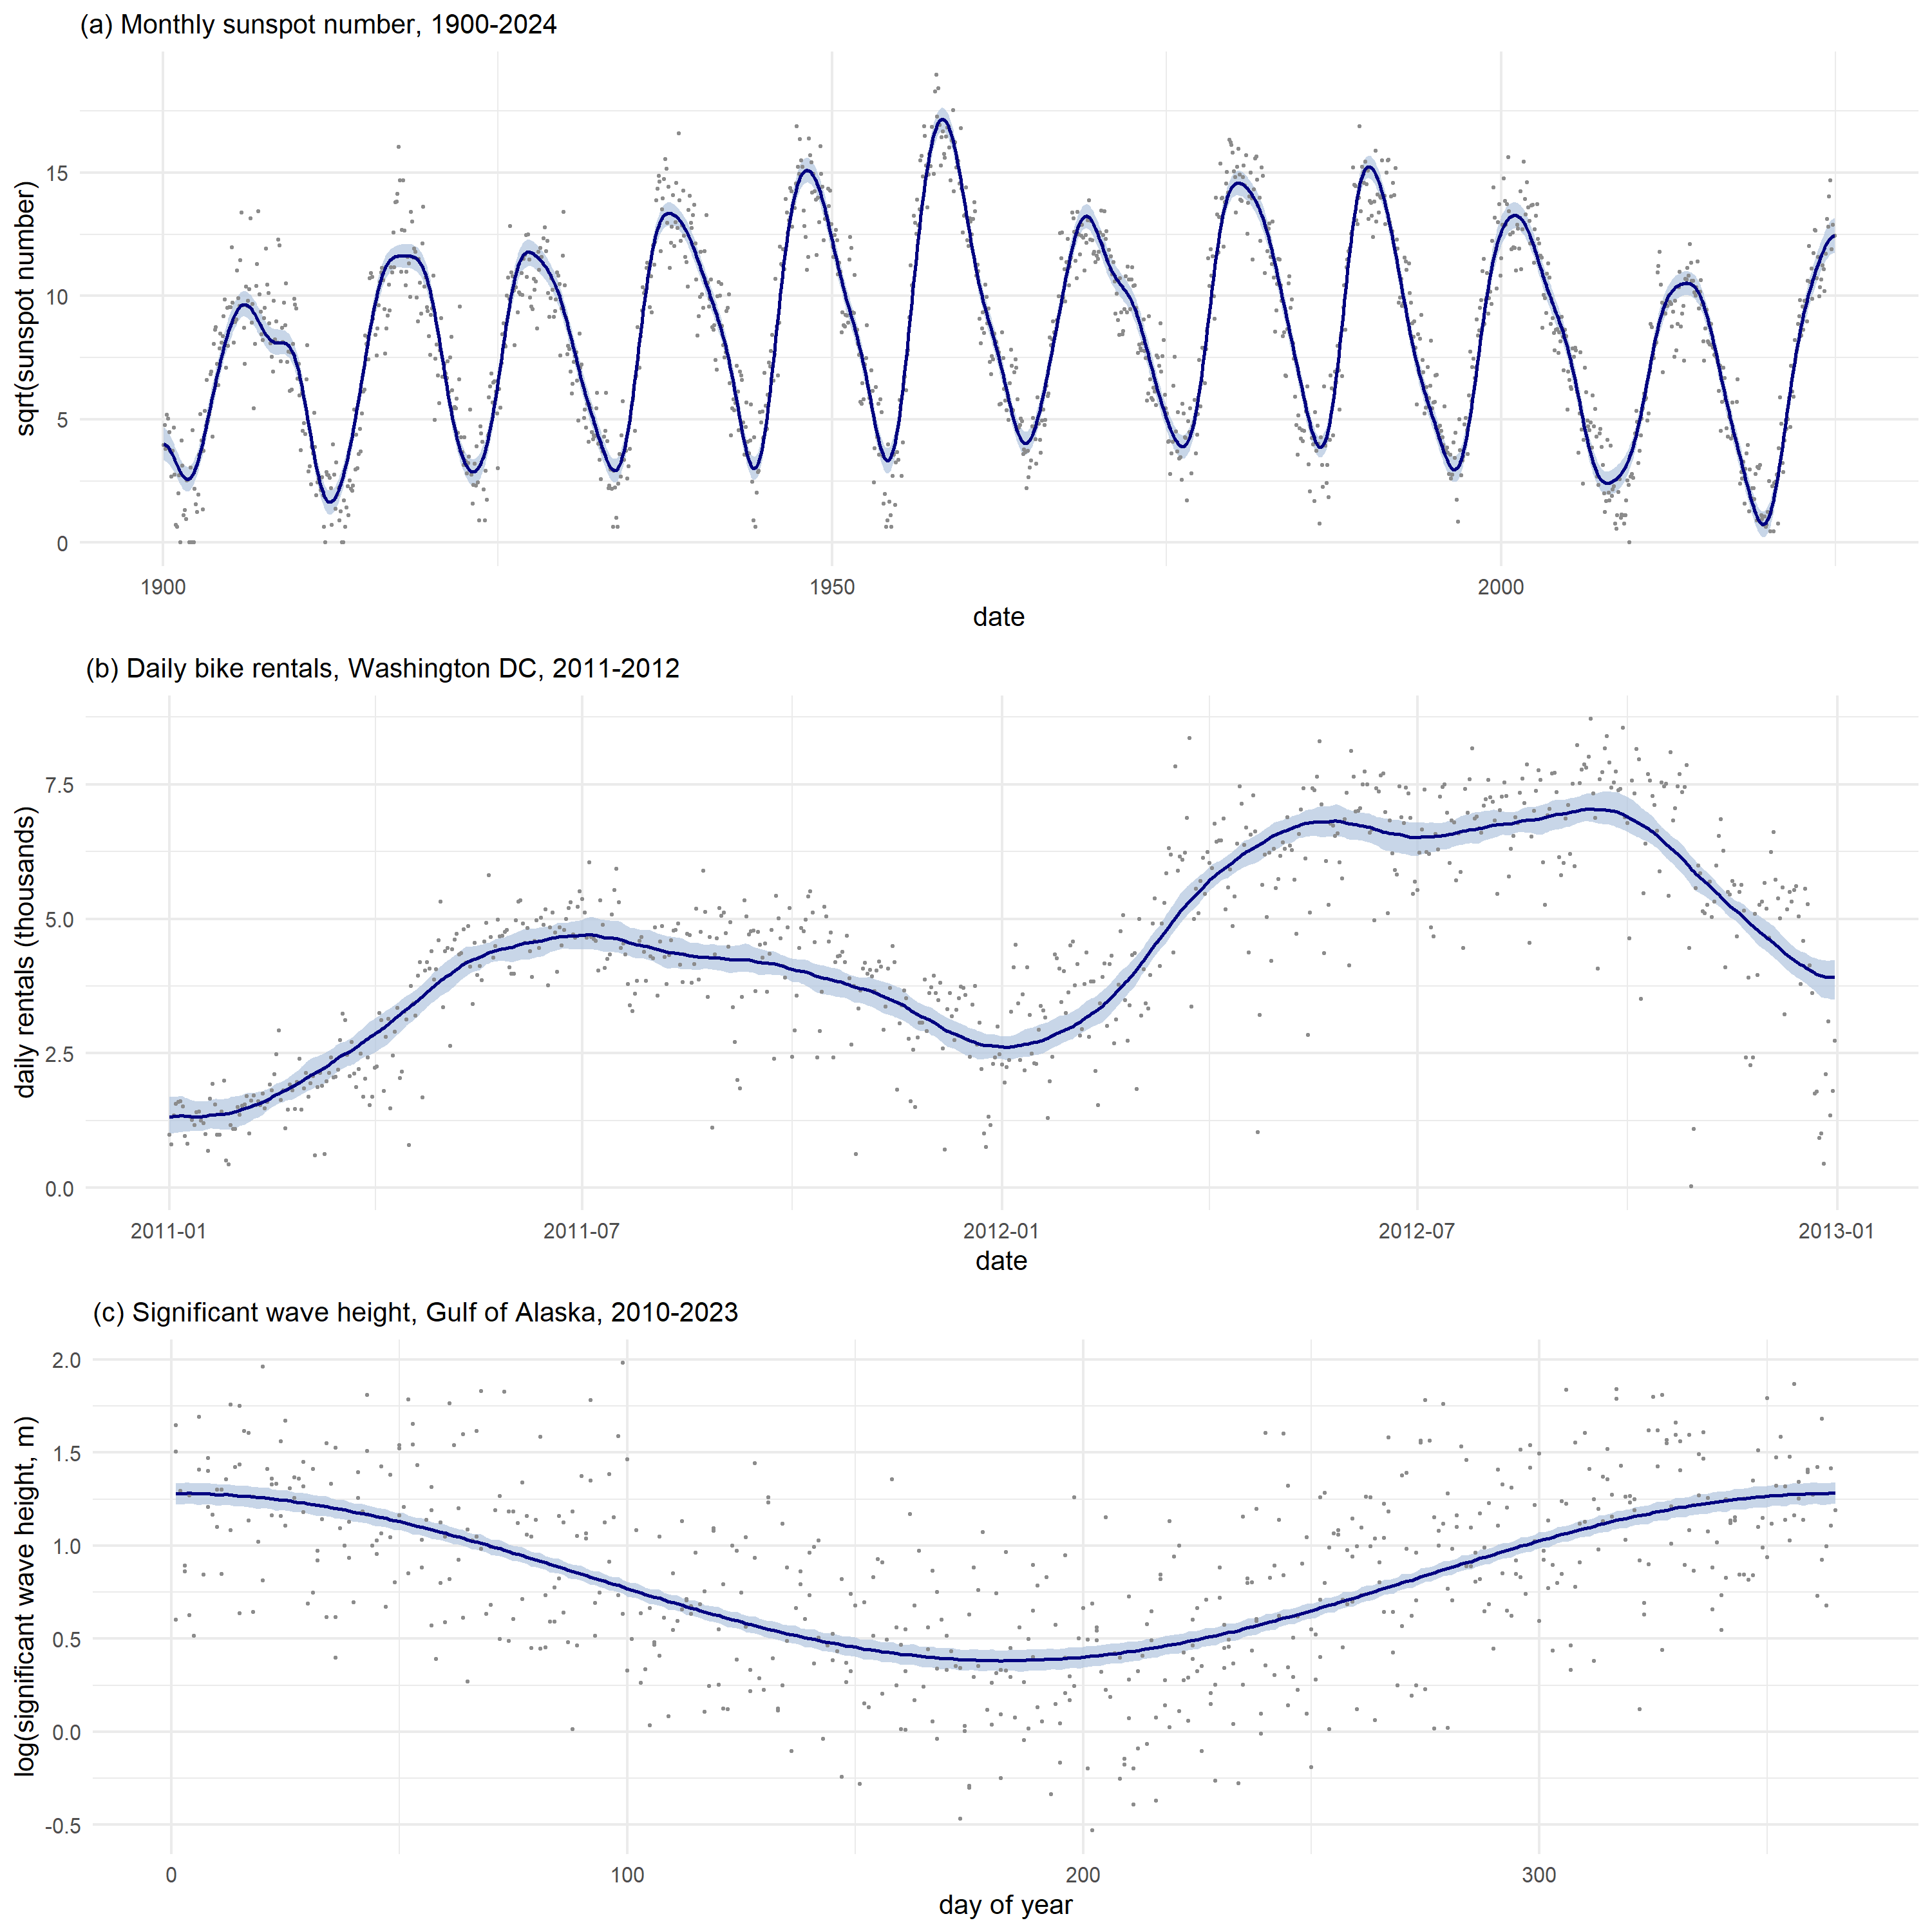
\includegraphics[width=\textwidth]{applications_fig.png}
\caption{Horseshoe fits with the dictionaries described in Section~\ref{sec:applications}, using the frequency cutoff $F_n=\lfloor n^{0.7}\rfloor$ and $\tau=F_n^{-2}$. Gray points are the data, curves are posterior means of the mean function, and shaded bands are pointwise $95\%$ credible bands for it.}
\label{fig:applications}
\end{figure}

Figure~\ref{fig:applications} shows the three fits. In each case the posterior mean is smooth and follows the systematic part of the series rather than its scatter:
\begin{itemize}
\item for the sunspots, the solar cycles with their varying length and amplitude;
\item for the bike rentals, the growth of the system over the two years together with its seasonal pattern;
\item for the wave heights, a single annual cycle, with rough winters and calm summers.
\end{itemize}
No series required its own choice of the number of terms: the dictionary size and the global scale follow the same rule throughout, and the shrinkage prior selects the effective complexity of each fit.


